\documentclass{article}
\usepackage[utf8]{inputenc}
\usepackage{amsmath}
\usepackage{hyperref}
\usepackage[letterpaper, portrait, margin=1in]{geometry}
\usepackage{graphicx}
\graphicspath{{images/}}

\begin{document}
\title{Projeto Demonstrativo 2 - Calibração de câmeras}
\date{23-04-2016}
\author{Samuel Venzi Lima Monteiro de Oliveira\\14/0162241\\samuel.venzi@me.com}

	\maketitle
	\pagenumbering{arabic}

	\section{Objetivos}
		\paragraph{}
		O objetivo deste processo é realizar um estudo sobre câmera e sua calibração. A partir desse estudo, desenvolver um método para calculo de dimensões de objetos dada a distância entre este e a câmera.
	\section{Introdução}
		\paragraph{}
		O uso de câmeras no âmbito da visão computacional é uma competência essencial devido às inúmeras aplicações práticas existentes. Tais aplicações vão desde câmeras de vigilância até carros autônomos, portanto é necessário saber sobre o funcionamento de câmeras e entender seus detalhes para que seja bem aplicada. Os principais pontos abordados neste estudo são a calibração de câmeras e, a partir disso, a avaliação do tamanho de objetos no \textit{frame} da imagem capturada.
		\paragraph{}
		A estrutura básica das câmeras atuais segue a estrutura consagrada pelos primeiros estudos feitos sobre capturas de imagens. O que essa estrutura permite é a entrada de luz por um orifício ou conjunto de lentes e sua projeção em um filme ou sensor que captura a imagem. As câmeras modernas utilizam lentes e sensores, e é importante entender como essas duas partes influenciam na maneira que deve se lidar com a manipulação de imagens dessas câmeras.
		\paragraph{}
		Com a introdução de lentes nas câmeras, foi possível a captura de imagens de muito melhor qualidade pois elas permitiam maior entrada de luz sem o desfoque da imagem, o que acontecia com o aumento do oríficio. Porém, a depender da qualidade de fabricação da lente, com elas ocorre o fenômeno da distorção que pode ser um grande problema para certas aplicações. No caso do uso de sensores, certas caracteríscas são importantes serem conhecidas, como seu tamanho e o tamanho de seus \textit{pixels}.
		\paragraph{}
		A calibração da câmera tem como função anular certas distorções da imagem que possam ocorrer por sua parte física. Portanto, alinhando hardware e software pode-se ter a representação mais fiel possível e a partir dessa representação retirar informações de interesse.
		\begin{center}
			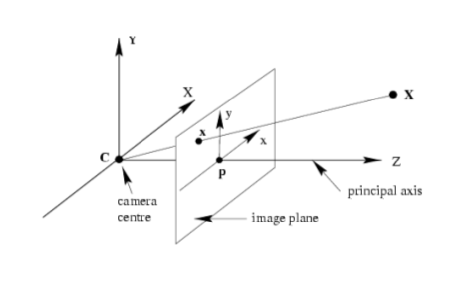
\includegraphics[scale=0.4]{CalibrationVariables}\\
			Figura 2.1
		\end{center}
		\paragraph{}
		Na figura 2.1 pode-se verificar algumas das variáveis de calibração. O sistema de referência é o plano da imagem, chamado também de frame e as coordenadas dos pixels no frame são dados por um par ordenado (x,y). 
		\paragraph{}
		A partir de estudos, são extraídas informções sobre a câmera, como seus parâmetros intrínsecos e extrínsicos. Onde os parâmetros intrínsecos caracterizam propriedades óticas, geométricas e digitais da câmera, além de sua distorção.
	\section{Materiais e Metodologia}
		\subsection{Materiais}
			\begin{itemize}
			\item Computador com ambiente Linux (Ubuntu)
			\item Câmera própria do computador
			\item OpenCV
			\item Esfera com 6cm de diâmetro
			\end{itemize}
		\subsection{Metodologia}
			\paragraph{}
			Antes de mexer com a câmera em si, foi criada uma aplicação que captura o clique do mouse em dois pontos arbitrários da janela, desenha um linha e calcula a distância em \textit{pixels} entre eles. O programa primeiramente cria uma imagem genérica, foi escolhida uma completamente preta, e com o uso de funções do OpenCV, captura e desenha uma linha ente dois pontos. Após isso ele calcula a distância Euclidiana Bidimensional.
			\paragraph{}
			Após isso, com a utilização de um programa de calibração já pronto, foi feita a calibração da câmera. Esse procedimento é muito importante e deve ser feito de forma extremamente cuidadosa. O procedimento consiste em usar um padrão conhecido pelo programa e a partir de pequenas diferenças encontradas entre o padrão original e o capturado e aplicar correções à imagem. Neste experimento foi usado um padrão xadrez com quadrados com 28mm de lado. Ocorrem 30 capturas por calibração e com o tabuleiro, deve-se percorrer todo o espectro da imagem. Ao final desse procedimento, o programa gera dois arquivos XML, um com parâmetros de distorção e outro com parâmetros intrínsecos da câmera. Para garantir mais confiança nos resultados, o procedimento é repetido 5 vezes e os valores finais dos parâmetros são as respectivas médias das 5 medições.
			\paragraph{}
			Com a calibração feita, o programa de medição de distância foi adicionado ao programa da câmera já calibrada com os parâmetros finais. A partir disso, com um objeto com dimensões conhecidas, uma esfera com 6cm de diâmetro, e a distâncias pré-definidas foi medido tamanho em \textit{pixels} do objeto na imagem do computador, tanto para a imagem pura da câmera quanto para a imagem gerada pela calibração com o objetivo de comparar e analisar as diferenças.
		\section{Resultados}
			\paragraph{}
			Uma calibração de câmera rende dois arquivos XML com os parâmetros de distorção e parâmetros intrínsecos. Então para as 5 calibrações feitas, temos 2 arquivos para cada. As médias e desvios padrões calculados seguem nas tabelas 1 e 2.
			\begin{table}
				\caption{média dos parâmetros de distorção}
				\centering
				\begin{tabular}{c c c}
					parâmetro & média & desvio padrão\\
					\hline\hline
					1 & -2.062004 & 1.766675\\
					2 & -49.042293 & 108.069947\\
					3 & 0.085966 & 0.043708\\
					4 & -0.071295 & 0.022296\\
				\end{tabular}
			\end{table}
			\begin{table}
				\caption{média dos parâmetros intrínsecos}
				\centering
				\begin{tabular}{c c}
					parâmetro & média \\
					\hline\hline
					1 & 259.555691\\
					2 & 326.942780\\
					3 & 2703.41079\\
					4 & 241.911987\\
				\end{tabular}
			\end{table}
			\paragraph{}
			Com um \textit{grid} de 8 retângulos montado no \textit{frame} da câmera, a medida em pixels da esfera em cada uma das células para distâncias diferentes é mostrado na tabela 3 (\textit{undistort}) e 4 (\textit{raw}). (Cada medida foi feita 5 vezes.)
			\begin{table}
				\caption{média dos tamanhos da esfera para cada célula da janela Undistort}
				\centering
				\begin{tabular}{c c c c c}
				distância (m)& 0,2 & 0,8 & 1,5 & 3,0\\
				\hline\hline
				cell 1 & 166,497800 & 52,817740 & 27,505600 & 12,539450\\
				cell 2 & 135,159200 & 45,854020 & 24,380280 & 11,625720\\
				cell 3 & 129,121500 & 46,160020 & 24,275700 & 11,299180\\
				cell 4 & 139,846400 & 49,413517 & 24,263340 & 10,907740\\
				cell 5 & 172,203600 & 60,735533 & 29,371820 & 14,194814\\
				cell 6 & 135,622800 & 49,419720 & 26,814820 & 10,498260\\
				cell 7 & 157,069400 & 47,414640 & 28,070640 & 10,477860\\
				cell 8 & 186,630800 & 50,993100 & 26,623400 & 11,557340\\
				
				\end{tabular}
			\end{table}
			\begin{table}
				\caption{média dos tamanhos da esfera para cada célula da janela Raw}
				\centering
				\begin{tabular}{c c c c c}
				distância (m)& 0,2 & 0,8 & 1,5 & 3,0\\
				\hline\hline
				cell 1 & 139,659800 & 42,586260 & 22,792967 & 10,834630\\
				cell 2 & 132,449800 & 45,288380 & 23,637840 & 11,809080\\
				cell 3 & 122,982833 & 46,880040 & 24,240880 & 10,907740\\
				cell 4 & 129,864000 & 47,007250 & 24,226620 & 10,924880\\
				cell 5 & 157,237000 & 53,756267 & 27,121240 & 12,721157\\
				cell 6 & 134,815200 & 50,243360 & 27,056580 & 10,056534\\
				cell 7 & 158,016800 & 47,215040 & 26,623280 & 10,886160\\
				cell 8 & 180,105600 & 51,005650 & 25,935867 & 11,511780\\
				\end{tabular}
			\end{table}
	\section{Discussão e Conclusões}
		\subsection{Discussão}
		\paragraph{}
		Devido dificuldade apresentada no processo de calibração da câmera, os parâmetros gerados não foram os melhores possíveis e os resultados apresentados se basearam em imagens levemente distorcidas, principalmente nas bordas. Esse efeito pode ser visto, principalmente, na comparação entre os tamanhos em pixels da esfera na saída \textit{raw} e na saída \textit{undistort} (calibrada). Nas células 1, 4, 5 e 8 (células dos 4 cantos de vídeo), apresenta-se uma maior diferença entre os tamanhos, onde a imagem estava mais distorcida. Portanto para melhor refletir o tamanho do objeto, recomenda-se que ele esteja localizado no centro do \textit{frame} da câmera.
		\paragraph{}
		Um dos possíveis motivos para uma calibração mal-sucedida pode ser alguma irregularidade na confecção por parte do fabricante, já que a câmera utilizada é embutida em um computador e, portanto, deve ser barata. Outro aspecto importante notar é que a calibração é feita manualmente, portanto é extremamente difícil alcançar a precisão desejável para que se possa garantir uma calibração razoável.
		\subsection{Conclusões}
		\paragraph{}
		Com o que foi exposto, é possível perceber a real dificuldade de calibrar câmeras por ser um processo extremamente suscetível a erros do calibrador. Também é possível concluir que a qualidade de fabricação da câmera é um fator importante.
	\section{Bibliografia}
		\paragraph{}
		A bibliografia principal utilizada foram sites da internet. \newline
		\paragraph{} \url{http://docs.opencv.org/3.1.0/d4/d32/classcv_1_1__InputArray.html#a0bd4ebf9eddfba4e1f8b5c3a099fa0ec&gsc.tab=0}
		\paragraph{}
		\url{http://docs.opencv.org/3.0.0/da/d54/group__imgproc__transform.html#ga7dfb72c9cf9780a347fbe3d1c47e5d5a}
		\paragraph{}
		\url{http://docs.opencv.org/3.0-rc1/dd/d74/tutorial_file_input_output_with_xml_yml.html}
		\paragraph{}
		\url{http://docs.opencv.org/2.4/modules/core/doc/drawing_functions.html#line}
		\paragraph{}
		\url{http://answers.opencv.org/question/38576/return-coordinate-values-from-mouse-callback-function-and-save-values-to-txt/}
		
		  
\end{document}